\documentclass{standalone}
\usepackage{pgfplots}
\pgfplotsset{compat=1.17}
\usetikzlibrary{arrows.meta}

% Define colors
\definecolor{myblue}{RGB}{0,0,255}
\definecolor{mygreen}{RGB}{0,255,0}
\definecolor{myred}{RGB}{255,0,0}

\begin{document}
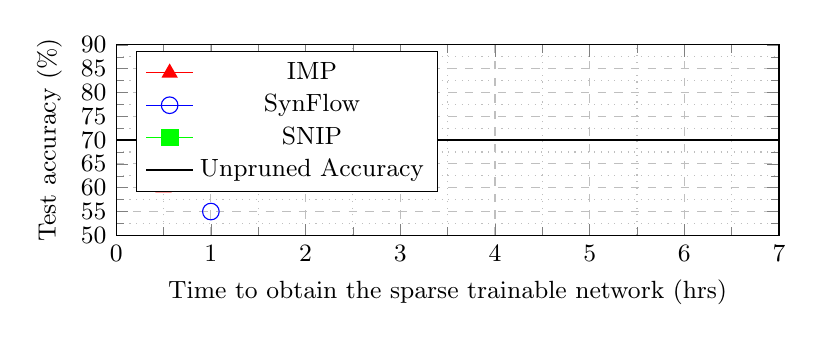
\begin{tikzpicture}
\begin{axis}[
    xlabel={Time to obtain the sparse trainable network (hrs)},
    ylabel={Test accuracy (\%)},
    xmin=0, xmax=7,
    ymin=50, ymax=90,
    ytick={50,55,60,65,70,75,80,85,90},
    xtick={0,1,2,3,4,5,6,7},
    grid=both,
    minor tick num=1,
    major grid style={dashed, gray!50},
    minor grid style={dotted, gray!50},
    legend pos=north west,
    legend style={draw=black, fill=white, font=\small},
    width=10cm, height=4cm,
    tick label style={font=\small},
    label style={font=\small}
]

% IMP
\addplot[
    color=myred,
    mark options={solid, myred, scale=1.5},
    mark=triangle*,
    ]
    coordinates {(0.5,60) (2,75)};
\addlegendentry{IMP}

% SynFlow
\addplot[
    color=myblue,
    mark options={solid, myblue, scale=1.5},
    mark=o,
    ]
    coordinates {(1,55)};
\addlegendentry{SynFlow}

% SNIP
\addplot[
    color=mygreen,
    mark options={solid, mygreen, scale=1.5},
    mark=square*,
    ]
    coordinates {(2.5,65)};
\addlegendentry{SNIP}

% Unpruned Accuracy
\addplot[
    thick,
    black
    ]
    coordinates {(0,70) (7,70)};
\addlegendentry{Unpruned Accuracy}

\end{axis}
\end{tikzpicture}
\end{document}